\chapter{Analyse av samvariasjon}
\label{kap:samvariasjon} % Opprinnelig kapittelnr: 9

Mange statistiske undersøkelser tar sikte på å avdekke
samvariasjon og mulige årsakssammenhenger mellom variable.
Vi har to hovedtyper variable: {\em kategorivariable} og 
{\em målevariable}. I en undersøkelse som angår individer er
kjønn, boregion og holdning (negativ, indifferent, positiv) alle
kategorivariable, mens reaksjonsevne, alder og puls er målevariable.
Ofte nyttes andre betegnelser: Kategorivariable kalles gjerne {\em kjennetegn}
i spørre\-skjema\-under\-søkelser og {\em faktorer} i andre sammenhenger.
I litteraturen findeles ofte variabeltypene ytterligere.
Kategorivariable deles i tre typer: Variable med to kategorier (som kjønn)
kalles {\em dikotome variable}, de med flere uordnede kategorier (som bosted)
kalles {\em nominale variable}, de med flere ordnede kate\-gorier (som holdning)
kalles {\em ordinale variable}.

Vi vil i dette kapitlet ta for oss analyse av samvariasjon, først
for kategorivariable og avslutningsvis for målevariable.
Vi vil også diskutere farer for slutningsfeil, både når det gjelder
tilfeldigheters rolle og påståtte årsakssammenhenger.
For målevariable blir dette tema også bli belyst i Kapittel 12.

\section{Kryssklassifiserte hyppigheter}
Anta at vi utfører en  undersøkelse der vi registrerer antall objekter
eller individer som faller i hver av flere mulige kategorier, bestemt
ved at observasjonene kryssklassifiseres mhp. to eller flere kjennetegn
(kategorivariable).\\

\begin{eksempel}{Kunder}
I en undersøkelse omkring kundene i et varehus kan man tenke seg å
studere en rekke kjennetegn for ekspederte kunder, eksempelvis kjønn,
yrkesstatus, inntekt, kundeforhold, varenes kostende og betalingsform.
For de ulike kjennetegn kan vi tenke oss følgende kategorier:  kjønn
(mann, kvinne), yrkesstatus (yrkesaktiv eller ikke), inntekt (lav, høy),
kundeforhold (fast, tilfeldig), varenes kostende (lav, middels, høy),
betalingsform (kontanter, kort, annen).  Brukes denne listen av
kategorier for hvert kjennetegn vil hver kunde kunne klassifiseres i en
av $2\cdot 2\cdot 2\cdot 2\cdot 3\cdot 3 = 144$ mulige kategorier.
I praksis kan en være interessert i å bruke flere (eller færre)
kategorier for noen av kjennetegnene, eksempelvis inntekt (lav, middels,
høy), betalingsform (kontanter, annen).  Vi kan også være
interessert i flere, færre eller andre kjennetegn.  Hvilke kjennetegn
og kategorier som brukes, vil avhenge av formålet med undersøkelsen,
samt muligheten for og kostnadene ved å innhente de nødvendige
opplysninger.
\end{eksempel}

Resultatet av undersøkelser med kryssklassifiserte hyppigheter
gis ofte i form av såkalte  {\em kontingenstabeller}.
Den enkleste situasjonen har vi når det foreligger to kjennetegn 
som hvert innbyr til klassifisering i to kategorier.  Våre data er da
gitt i form av en $2\times 2$ tabell.\\

\begin{eksempel}{Kortbruk}
La situasjonen være som i Eksempel 1.  I alt $n$=250 utvalgte kunder
har fylt ut et spørreskjema som skal sette oss i stand til å
studere eventuelle sammenhenger mellom en rekke kjennetegn.  La oss
først klassifisere m.h.t. kjennetegnene betalingsform og kjønn.
Anta at annet betalingsmiddel enn kontanter i dette eksemplet alltid
er kort, og at resultatet er i Tabell~\ref{tab:data}.

\begin{table}[h]  \centering 
\begin{tabular}{l|cc|c}
       & Kontanter & Kort & Sum  \\ \hline
Kvinne &    85     &  55  & 140   \\
Mann   &    50     &  60  & 110   \\ \hline
Sum    &   135     & 115  & 250   \\ \hline
\end{tabular}
\caption{Data}
\label{tab:data} % Tabell_1
\end{table}

\noindent Ønsker vi en tabell over de relative hyppigheter kan vi dividere
alle tall i tabellen med antall observasjoner $n$=250, som gir Tabell~\ref{tab:rel_hyppigheter}.

\begin{table} \centering
\begin{tabular}{l|cc|c}
       & Kontanter & Kort & Sum  \\ \hline
Kvinne &    0.34   & 0.22 & 0.56 \\ 
Mann   &    0.20   & 0.24 & 0.44 \\ \hline
Sum    &    0.54   & 0.46 & 1.00 \\ \hline
\end{tabular}
\caption{Relative hyppigheter}
\label{tab:rel_hyppigheter} % Tabell_2
\end{table}

\noindent Av dette kan det være fristende å konkludere at kundekretsen 
består av flest kvinner og at kundekretsen viser større 
tilbøyelighet til å bruke kontanter enn kort.  Av interesse er
også de linjevise relative hyppighetene i Tabell~\ref{tab:linjevise} (med to desimaler),
som antyder at korttilbøyeligheten er betydelig mindre
blant kvinner enn blant menn.
\end{eksempel}

\begin{table} \centering 
\begin{tabular}{l|cc|c}
       & Kontanter & Kort & Sum \\ \hline
Kvinne &   0.61    & 0.39 & 1.00 \\ 
Mann   &   0.45    & 0.55 & 1.00 \\ \hline
Sum    &   0.54    & 0.46 & 1.00 \\ \hline
\end{tabular}
\caption{Linjevise relative hyppigheter}
\label{tab:linjevise} % Tabell_3
\end{table}


La oss imidlertid trå varsomt. Før vi i eksemplet framsetter
generelle konklusjoner angående kundekretsen, bør vi foreta en
vurdering om det observerte resultat kan skyldes tilfeldigheter og/eller
om det kan være andre forhold som tilslører bildet.  Til dette
kreves teori. 

\section{En modell for toveis-klassifikasjoner}

La oss betrakte våre observasjoner som utfall av et eksperiment, der
hvert utfall er beskrevet ved to eller flere kjennetegn (faktorer), med 
to eller flere kategorier (nivåer) for hvert kjennetegn.
Den enkleste situasjon er et såkalt $2\times 2$ klassifikasjon, dvs.
vi har to kjennetegn som begge tillater klassifisering i to kategorier,
slik at eksperimentet har $2\cdot 2=4$ mulige utfall. 
Et mulig $2\times 2$ eksperiment vil være dersom vi i Eksempel 1
observerer en tilfeldig kunde og registrerer kjønn og betalingsform
(kontanter, annen).  Dersom vi registrerer kjønn, yrkesstatus,
betalingsform (kontanter, kort, annen), har vi et $2\times 2\times 3$
eksperiment osv.

Vi vil i dette avsnittet se på en modell for toveis-klassifikasjoner.
Slike situasjoner forekommer ofte i praksis, og kunnskap om denne modellen
vil også kunne være til hjelp for forståelsen av mer kompliserte
situasjoner, f.eks. ved analyse av delproblemer som angår bare to
kjennetegn. La oss bruke følgende notasjon:

Gitt to kjennetegn $e$ og $f$, der $e$ klassifiseres i $r$ kategorier 
$e_1,e_2,\ldots ,e_r$ og $f$ klassifiseres i $s$ kategorier 
$f_1,f_2,\ldots ,f_s$. Vi har da $r\cdot s$ mulige utfall $(e_i,f_j)$
$i=1,2,\ldots r$; $j=1,2,\ldots s$. La $p_{ij}$ være sannsynligheten
for utfallet $(e_i,f_j)$ . En slik $r\times s$ situasjon kan oversiktlig
presenteres ved en toveistabell med $r$ rader og $s$ søyler.
For $2\times 2$ situasjonen med 4 utfall ser tabellen ut som Tabell~\ref{tab:modell2x2}.

\begin{table} \centering 
\begin{tabular}{l|cc|c}
      &  $f_1$    &  $f_2$   &  Sum  \\ \hline
$e_1$ &  $p_{11}$ &  $p_{12}$& $p_{1\cdot}$  \\ 
$e_2$ &  $p_{21}$ &  $p_{22}$& $p_{2\cdot}$ \\  \hline
Sum   & $p_{\cdot 1}$&$p_{\cdot 2}$&   1    \\ \hline
\end{tabular}
\caption{Modell for $2\times 2$ eksperiment}
\label{tab:modell2x2} % Tabell_4
\end{table}

La $p_{i\cdot}$ ; $i=1,2,\ldots ,r$ være de marginale sannsynligheter
for de $r$ kate\-goriene for kjennetegnet $e$, og
$p_{\cdot j}$ ; $j=1,2,\ldots ,s$ være de marginale sannsynligheter
for de $s$ kategoriene for kjennetegnet $f$.
I tabellen finnes disse ved å summere henholdsvis radene og søylene.
Merk at prikken mar\-kerer at vi har summert $p_{ij}$ over de fotskrifter som
kan være på prikkens plass, dvs. $p_{1\cdot } = p_{11} + p_{12}$
osv.

En mulig hypotese vil være at de to kjennetegnene er uavhengige,
 ifølge definisjonen av uavhengighet skjer dette når
\[    p_{ij} = p_{i\cdot } \cdot  p_{\cdot j}            \]
for alle $i=1,2,\ldots ,r$ og $j=1,2,\ldots ,s$, dvs. når sannsynlighetene
for alle utfall i tabellen er lik produktet av de tilhørende marginale
sannsynlighetene (se Kapittel 4.5 om uavhengighet og produktmodeller). 

De betingede sannsynligheter for kjennetegnet $f$ gitt at $e_i$ observeres,
er for $i=1,2,\ldots ,r$ gitt ved

\[ P(f_j\mid e_i)=P((e_i,f_j))/P(e_i)=p_{ij}/p_{i\cdot} \mbox{\ \ \ }
                                                     j=1,2,\ldots ,s   \]
dvs. hver rad divideres med marginaltallet til høyre. Ved uavhengighet
blir $P(f_j\mid e_i)=P(f_j)=p_{\cdot j}$, slik at alle disse radbrøkene
er lik marginalraden i bunnen av tabellen. Tilsvarende blir hver søyle ved
divisjon av marginaltallet i bunnen av tabellen lik marginalraden til høyre.
Konkret betyr det at uansett hvilken kategori vi observerer for det ene
kjennetegnet, så vil alle sannsynligheter for det andre være uendret.

Dersom betingelsen for uavhengighet ikke er oppfylt, sier vi at kjennetegnene
er avhengige eller viser {\em samvariasjon}. Samvariasjon kan anta mange ulike 
former. Dersom kategoriene er ordinale, dvs. kan ordnes i en naturlig
rekkefølge, kan vi tale om positiv samvariasjon. Dette betyr at
kategorikombinasjoner høy/høy og lav/lav  gjennomgående
har større sannsynlighet enn høy/lav og lav/høy for de to kjennetegn.
Negativ samvariasjon betyr at kombinasjonene høy/lav og lav/høy
gjennomgående har større sannsynlighet enn høy/høy og lav/lav.

Positiv samvariasjon betyr grovt sagt at det  i toveistabellen er mer
sannsynlighet rundt diagonalen fra nordvest til sørøst enn rundt
diagonalen fra sørvest til nordøst.
I $2\times 2$ situasjonen kan alltid kjennetegnene oppfattes som ordinale
(hvorfor?), og avhengighet kan uttrykkes ved det såkalte 
{\em kryssproduktforholdet} $K=p_{11}p_{22}/p_{12}p_{21}$, som ved
uavhengighet er lik 1, og ved positiv (negativ) samvariasjon er større 
(mindre)  enn 1.

La oss nå tenke oss at eksperimentet er utført $n$ ganger uavhengig av 
hverandre, og at vi observerer antall ganger hvert utfall inntreffer. La

\[ X_{ij}= \mbox{antall ganger utfallet $(e_i,f_j)$ observeres.} \]
Resultatene av et slikt $r\times s$ eksperiment kan oversiktlig
presenteres ved en toveis kontingenstabell med $r$ rader og $s$ søyler.
For $2\times 2$ situasjonen med 4 utfall ser tabellen ut som Tabell~\ref{tab:observasjoner2x2}.

\begin{table}[h] \centering 
\begin{tabular}{l|cc|c}
      &  $f_1$    &  $f_2$   &  Sum  \\ \hline
$e_1$ &  $X_{11}$ &  $X_{12}$& $X_{1\cdot}$  \\ 
$e_2$ &  $X_{21}$ &  $X_{22}$& $X_{2\cdot}$  \\  \hline
Sum   & $X_{\cdot 1}$&$X_{\cdot 2}$&   $n$  \\ \hline
\end{tabular}
\caption{Observasjoner av $2\times 2$ eksperiment}
\label{tab:observasjoner2x2} % Tabell_5
\end{table}

De marginale antall i hver av kategoriene for kjennetegnet $e$ betegner vi
$X_{i\cdot}$ ; $i=1,2,\ldots ,r$, og  de marginale antall i hver av
kategoriene for kjennetegnet $f$ betegner vi $X_{\cdot j}$ ; $j=1,2,\ldots ,s$.
I tabellen finnes disse ved å summere henholdsvis radene og søylene.
Prikken markerer at vi har summert over de fotskrifter som kan være på
prikkens plass, i tabellen $X_{1\cdot } = X_{11} + X_{12}$ osv., slik at
notasjonen samsvarer med den for sannsynlighetene.

De naturlige estimatorene for utfallssannsynlighetene i toveis-tabellen er de
tilsvarende observerte relative hyppigheter, dvs. 

\[ \hat{p}_{ij}=X_{ij}/n \]
og for  de marginale sannsynlighetene

\[ \hat{p}_{i\cdot}=X_{i\cdot}/n \mbox{\ \ \ \ }
                           \hat{p}_{\cdot j}=X_{\cdot j}/n \]
Av forutsetningen om n uavhengige observasjoner følger , ved å la
utfallet $(e_i,f_j)$ bety suksess, at $X_{ij}$ er
binomisk fordelt $(n,p_{ij})$. 
Dette betyr at $EX_{ij}=np_{ij}$, som viser at estimatorene ovenfor er
forventningsrette. 

Estimatorer for de ulike betingede sannsynligheter gir seg også,
henholdsvis de linjevise og kolonnevise relative hyppigheter (jfr. Tabell~\ref{tab:linjevise}). 

Dersom vi antar at kjennetegnene $e$ og $f$ er uavhengige, vil en mer
naturlig estimator for $p_{ij}$ være

\[ \check{p}_{ij}=\hat{p}_{i\cdot}\cdot \hat{p}_{\cdot j} \]
og hvis $\check{p}_{ij}$ gjennomgående ikke er mye forskjellig fra
$\hat{p}_{ij}$, er det grunn til å tro at kjennetegnene er (tilnærmet)
uavhengige. Dette er altså tilfelle når de relative hyppighetene
(Jfr. Tabell~\ref{tab:rel_hyppigheter}) er tilnærmet lik produktet av de tilhørende marginale
hyppighetene, dvs. når

\[  \frac{X_{ij}}{n}\approx \frac{X_{i\cdot}}{n}\cdot \frac{X_{\cdot j}}{n} \]
For at situasjonen i Eksempel 2 skal beskrives ved  modellen ovenfor, må vi
oppfatte observasjonene for de 250 kundene som $n=250$ uavhengige rea\-lisasjoner
av et $2\times 2$ eksperiment, med samme sannsynlighet for at hver (tilfeldig)
kunde faller i de ulike kategoriene. Dette er rimelig dersom kundene utgjør
et tilfelig utvalg fra en stor kundekrets.
De relative hyppighetene i Tabell~\ref{tab:rel_hyppigheter} vil da kunne oppfattes som estimater for
de teoretiske sannsynlighetene i $2\times 2$-modellen. Vi ser at
multiplikasjonsegenskapen ovenfor langt fra er oppfylt i dette tilfellet,
som igjen antyder at kjennetegnene kjønn og kortbruk kan være avhengige.

Under de forutsetningene som er nevnt ovenfor, vil den simultane fordeling
til observasjonene i kontingenstabellen (Tabell~\ref{tab:observasjoner2x2}) være såkalt
multinomisk fordelt (jfr. Kapittel 6.8).  Ytterligere egenskaper ved
estimatorene og mulige aktuelle testmetoder kan derfor studeres på
grunnlag av denne fordeling.

I de fleste anvendelser ønsker vi å
trekke konklusjoner om en avgrenset populasjon på $N$ elementer
(ofte individer) som kan klassifiseres mhp. to kjennetegn $e$ og $f$.
Anta at det i populasjonen er $N_{ij}$ individer som vil kunne 
klassifiseres i kategori ($e_i, f_j$).  Andelen slike individer er
$N_{ij}/N$.  Vi antar at disse andelene er ukjente og at vi trekker et
utvalg på $n$ individer fra populasjonen med sikte på å
anslå andelene, evt. si noe om samvariasjonen mellom
kjennetegnene i populasjonen.  Ved trekning med tilbakelegging vil en 
kunne betrakte hver trekning som et forsøk der vi har sannsynlighet
$p_{ij} = N_{ij}/N$ for utfallet $(e_i, f_j)$, slik at modellen ovenfor
gjelder.  Når slike utvalg i praksis trekkes uten tilbakelegging 
blir modellen en tilnærmelse, men dersom $n$ er liten i forhold til $N$ 
(som regel er dette tilfelle), er forskjellen uten betydning, og modellen
blir derfor brukt også i slike situasjoner istedenfor mer 
kompliserte (flervariable hypergeometriske) modeller. Ofte er populasjonen
ikke klart avgrenset, noe som antakelig vil være tilfelle med kundekretsen
i Eksempel 2. \\

\begin{eksempel}{Avstemming}
I en undersøkelse om aktiviteten blant medlemmer i en yrkesorganisasjon
er det utsendt spørreskjemaer til et tilfeldig utvalg av medlemmene
og i alt $n$=200 utfylte skjemaer foreligger til analyse.  Vi er bl.a.
interessert i kjennetegnet kjønn og om vedkommende avga stemme over siste
tariff-forslag eller ikke.  Anta at resultatet ble som i Tabell~\ref{tab:observasjoner2}.

\begin{table}[h] \centering 
\begin{tabular}{l|cc|c}
       & Stemte & Stemte ikke & Sum  \\ \hline
Mann   &    86  &  34         & 120   \\
Kvinne &    64  &  16         &  80   \\ \hline
Sum    &   150  &  50         & 200   \\ \hline
\end{tabular}
\caption{Observasjoner}
\label{tab:observasjoner2} % Tabell_6
\end{table}

For å undersøke om kjennetegnene kjønn og stemmetilbøyelighet
med rimelighet kan sies å være uavhengige, kan vi se på
Tabell~\ref{tab:rel_hyppigheter2}  der vi har beregnet de relative hyppighetene, samt
påført de tilhørende produkter av de marginale hyppighetene i
parentes.

\begin{table}[h] \centering 
\begin{tabular}{l|ll|l}
       & Stemte       & Stemte ikke  & Sum  \\ \hline
Mann   &  0.43 (0.45) &  0.17 (0.15) & 0.60   \\
Kvinne &  0.32 (0.30) &  0.08 (0.10) & 0.40  \\ \hline
Sum    &  0.75        &  0.25        & 1.00   \\ \hline
\end{tabular}
\caption{Relative hyppigheter}
\label{tab:rel_hyppigheter2} % Tabell_7 
\end{table}
Vi ser at de observerte hyppigheter ikke er mye forskjellig fra produktet
av de marginale hyppighetene, og det synes lite rimelig å påstå
at stemmetilbøyeligheten avhenger av kjønn (på tross av at de
linjevise relative hyppighetene viser at 72\% av mennene og hele 80\%
av kvinnene stemte).  Dersom vi aksepterer tanken om uavhengige kjennetegn,
vil det være naturlig på grunnlag av de observerte data å
bruke tallene i parentes som sannsynligheter i en eventuell modell.
Disse sannsynlighetene skal da representere sjansene for at et tilfeldig
valgt medlem faller i de ulike kategoriene.
\end{eksempel}


\section{Testing av uavhengighet og \newline mål for samvariasjon}

I praksis vil to kjennetegn bli betraktet som uavhengige dersom
produktet av de marginale hyppighetene ikke avviker altfor mye fra
hyppighetene av hvert utfall.  I motsatt fall betraktes kjennetegnene
som avhengige. Dette betyr samvariasjon, men ikke nødvendigvis noe direkte
årsaksforhold.  Spørsmålet er imidlertid hvor store avvik
vi kan tilskrive tilfeldigheter og likevel betrakte de to kjennetegnene
som uavhengige.  Det er vanskelig å gi noe entydig
svar på dette, det vil bl.a. avhenge av hvilken bruk vi vil gjøre
av resultatet.  I en del situasjoner med en viss avhengighet mellom
kjennetegnene, vil avhengigheten være såpass liten at det er
hensiktsmessig å holde på uavhengighet, fordi dette er en enklere
modell, og det ikke har praktiske konsekvenser å anta noe annet.

La oss formulere situasjonen som et hypotese\-testingsproblem, der
nullhypotesen er

\[ H_0 : \mbox{\ Kjennetegnene $e$ og $f$ er uavhengige }  \]
mot alternativet at kjennetegnene er avhengige. Mulig testobservator er:

\[ Q=\sum_{i=1}^{r}\sum_{j=1}^{s}
       \frac{{(X_{ij}-n{\hat{p}}_{i\cdot}{\hat{p}}_{\cdot j})}^2}
                           {n{\hat{p}}_{i\cdot}{\hat{p}}_{\cdot j}} .    \]
$Q$ kan oppfattes som mål for graden av avvik mellom de observerte
hyppigheter $X_{ij}$ og forventningen for tilfellet at kjennetegnene er 
uavhengige $np_{ij}=np_{i\cdot}p_{\cdot j}$, som vi estimerer med
$n{\hat{p}}_{i\cdot}{\hat{p}}_{\cdot j}$.

Store verdier av $Q$ indikerer at kjennetegnene er avhengige, og
spørsmålet er hvor stor $Q$ må være for at vi forkaster
nullhypotesen. Dersom situasjonen kan beskrives med toveis-modellen fra
forrige avsnitt og nullhypotesen om uavhengighet er riktig, kan det vises at
$Q$ for stor $n$  har fordeling som kan tilnærmes med kji-kvadratkurven
med frihetsgradtall $\nu = (r-1)\cdot (s-1)$ (Se Kapittel 7.7).\\

\begin{eksempel}{Vedtektsendring}
En større organisasjon vil undersøke holdningen til en foreslått
vedtektsendring blant medlemmene, spesielt er man interessert i om 
kjennetegnene alder og synspunkt er uavhengige eller ikke.  I alt er 
$n$=180 tilfeldig u\-tvalgte medlemmer spurt om saken.  Resultatene er
lagret som to kolonner i en datafil 'eks9.4' med følgende kodetall for de
to variablene : ALDER (1=under 30 år, 2=30 - 50 år, 3=over 50 år), 
SYNSPUNKT (1=negativ, 2=indifferent, 3=positiv). En analyse ga dette : 

\begin{center} \framebox[10cm]{\begin{minipage}{9cm}\rule{0cm}{0.5cm}
\tt
>> READ 'eks9.4' 'ALDER' 'SYN' \\
>> TABLE 'ALDER' 'SYN' ; CHISQUARE ; EXPECTED \\
\begin{tabular}{rrrrr}
        &   SYN 1 &   SYN 2 &   SYN 3 &   Total \\
ALDER 1 &      12 &      11 &      29 &      52 \\
        &    13.0 &    17.9 &    21.1 &         \\ 
ALDER 2 &      11 &      35 &      34 &      80 \\
        &    20.0 &    27.6 &    32.4 &         \\
ALDER 3 &      22 &      16 &      10 &      48 \\
        &    12.0 &    16.5 &    19.5 &         \\ 
 Total  &      45 &      62 &      73 &     180 \\ 
\multicolumn{5}{c}{TABLED : OBSERVED and EXPECTED COUNTS (below)}
 \end{tabular}\\     
CHISQUARE (D.F. = 4) = 24.8 (P-VALUE = 0.0001)\\
\mbox{}  \end{minipage} } \end{center}
Leseren kan bekrefte resultatene ved å bemerke at
\begin{eqnarray*}
 Q&=&{(12-13.0)}^2/13.0+{(11-17.9)}^2/17.9+{(29-21.1)}^2/21.1 \\
  &+&{(11-20.0)}^2/20.0+{(35-27.6)}^2/27.6+{(34-32.4)}^2/32.4 \\
  &+&{(22-12.0)}^2/12.0+{(16-16.5)}^2/16.5+{(10-19.5)}^2/19.5 \\
  &=&24.8
\end{eqnarray*}
 $P$-verdien til det observerte resultat blir (frihetsgrader 
$(3-1)\cdot (3-1)$=4)
\[       P= P_{H_0}(Q\geq 24.8)=0.0001                  \]

Merk at Tabell~\ref{tab:Kjikvadrat_Areal} i Appendiks~\ref{app:fordelngstabeller} ikke går tilstrekkelig langt, men gir at
$P < 0.001$. Uansett er dette så lite at det er grunn
til å påstå at holdning til vedtektsendringen viser
sammenheng med alder.  Merk at denne metoden ikke forteller hva denne
sammenheng består i, vi må da studere dataene nærmere.
Tallene  indikerer imidlertid at holdningen til endringen
går i negativ retning med økende alder.
\end{eksempel}

Vi ser at uttrykket som ble brukt til å teste uavhengighet ovenfor
har følgende form

\[  Q=\sum_{k=1}^m \frac{{(O_k-E_k)}^2}{E_k}     \]
der vi summerer over et antall kategorier $m$, og der $O_k$ og $E_k$ er
henholdsvis observert og (anslått) forventet antall i kategori nr. $k$.
Vi husker at den $Q$ som ble brukt til å teste om en modell var
realistisk i Kapittel 7.7 hadde samme struktur.  I virkeligheten er 
begge spesialtilfeller av en generell teori for testing av hypoteser i
såkalte multinomiske modeller (Se Kapittel 6.8).

For mange interessante hypoteser i slike modeller vil testobservatorer
av formen $Q$ ha sannsynlighetsfordeling som kan tilnærmes med
kjikvadratkurven med frihetsgradtall bestemt ut fra situasjonen.  Tester
basert på $Q$ kalles derfor {\em kjikvadrattester.}  Generelt vil
graden av tilnærming øke med $n$, men sannsynlighetene for utfall
i hver enkelt kategori bør heller ikke være for liten.  Som en 
tommelfingerregel brukes at alle $E_k$ bør være større enn 5.

I situasjoner der antall frihetsgrader er 1, slik tilfellet er i
$2\times 2$ situasjonen, viser det seg at tilnærmelsen til
kjikvadratkurven kan forbedres.  Istedenfor $Q$ ovenfor brukes

\[  Q=\sum_{k=1}^m \frac{{(\mid O_k-E_k\mid -0.5)}^2}{E_k}.     \]
Dette er en heltallskorreksjon analog med den vi bruker i 
normaltilnærmelsen, i litteraturen kalles dette {\em Yates korreksjon.}
Slik korreksjon har ingen betydning og kan sløyfes når $n> 50$.

I teorien ovenfor har vi forutsatt at $n$ var et gitt antall, mens alle de
andre tallene i den observerte tabell var tilfeldig bestemt.
I mange situa\-sjoner er den ene marginalen gitt på forhånd.
Det gjelder f.eks. dersom vi i Eksempel 2 bestemte oss for å spørre
ut 140 kvinner og 110 menn istedenfor å velge 250 kunder tilfeldig.
Situasjonen kan da betraktes som inferens om forskjeller mellom
sannsynligheter i to binomiske forsøksrekker, en teori som ble utviklet 
i Kapittel 7.6. Testen som ble omtalt der er imid\-ler\-tid likeverdig med
kjikvadrattesten, som derfor også kan brukes til å teste
hypotesen om at to sannsynligheter for to grupper observasjoner er like.

Merk at kjikvadrattesten kan også brukes når det er tale om
sannsynligheter for mer enn to kategorier for mer enn to grupper, f.eks.
dersom vi i Eksempel 4 bestemte oss for å spørre et gitt antall
i hver aldersgruppe (f.eks. 60 i hver), for så å teste om
sannsynlighetene for de ulike holdninger var like i de tre aldersgruppene.

Analyse av situasjoner der alle marginalene i en $2\times 2$ tabell er gitte,
blir tatt opp i Kapittel 10.3 i tilknytning til randomiserte eksperimenter.
I slike situasjoner kan vi begrunne enda en test som alternativ til
kjikvadrattesten i $2\times 2$ situasjonen.

I praksis studeres ofte endringer i holdninger eller adferd fra før
og etter et tiltak, og det er spørsmål om tiltaket virket.\\


\begin{eksempel}{Merkebytte}
La oss anta at det er gjennomført en reklamekampanje for en 
merkevare, og at data foreligger fra et forbrukerpanel på $n$=1000
personer som er spurt før og etter kampanjen (Tabell~\ref{tab:merkebytte}).

\begin{table} \centering 
\begin{tabular}{l|rr|r} 
Siste kjøp     &\multicolumn{2}{c|}{Siste kjøp etter kampanje}& \\  
før kampanje   &\multicolumn{1}{c}{Vårt merke (1)}&
                   \multicolumn{1}{c|}{Annet merke (2)} &  Sum  \\  \hline
Vårt merke (1)&        100          &       35         &  135  \\
Annet merke  (2)  &         65          &      800         &  865   \\ \hline
Sum               &        165          &      835         & 1000   \\ \hline
\end{tabular}
\caption{Merkebytte}
\label{tab:merkebytte} % Tabell_8
\end{table}
Det vil alltid være en viss overgang mellom merker.  At kampanjen ikke 
har noen virkning, kan oppfattes slik at sjansen for at en tilfeldig person
bytter fra vårt merke, er den samme som å bytte til vårt merke.
Med vår tidligere notasjon for $2\times 2$-tabeller, er 
nullhypotesen $p_{12} = p_{21}$, mens alternativet $p_{12} \neq p_{21}$
betyr endring, med $p_{21} > p_{12}$ i favør av vårt merke.

En egnet testmetode for denne situasjonen, {\em McNemars test}, er basert
på testobservatoren \footnote{Her er tallet 1 en korreksjon av
samme type som Yates korreksjon.}

\[ Q=\frac{{(\mid X_{12}-X_{21}\mid -1)}^2}{X_{12}+X_{21}}   \]
Denne er tilnærmet kjikvadratfordelt med 1 frihetsgrad når
nullhypotesen er riktig.  Nullhypotesen forkastes når $Q$ er 
stor, og våre data gir  

\[ Q=\frac{{(\mid 35-65\mid -1)}^2}{35+65}=8.41  \]
Dette gir $P=P_H(Q\geq 8.41) = 0.004$, som viser at nullhypotesen 
forkastes selv med forholdsvis lavt signifikansnivå.  Vi kan derfor
med rimelighet anta at den overvekt av overganger til vårt merke som er 
tilstede i våre data, ikke beror på tilfeldigheter. Om det 
er en varig effekt er en annen sak.
\end{eksempel}

Det er ofte ønskelig å kunne beregne et mål for styrken og om
mulig også retningen (positiv eller negativ) av en observert 
samvariasjon mellom to kjennetegn.  Dette vil ofte være tilfellet i
større undersøkelser der det ikke er plass til å gjengi alle
krysstabeller fullt ut.  En kan også ønske å sammenligne graden 
av samvariasjon i flere slike tabeller.  Videre kan det hende at selv om
en samvariasjon er statistisk signifikant, dvs. hypotesen om
uavhengighet er forkastet, så er likevel samvariasjonen uten
praktisk betydning.  Eksempelvis kan vi ha et ønske å predikere
et kjennetegn på grunnlag av observasjon av det andre kjennetegnet,
og det kan kreve en høy grad av samvariasjon for å være 
meningsfylt.  Merk forøvrig at det er først når vi har med
ordinale kjennetegn å gjøre, at det er aktuelt å tale om en
retning på samvariasjonen.

Det viser seg at det ikke fins noe allment akseptert mål for 
samvariasjon mellom kjennetegn, selv ikke i den enkle $2\times 2$
situasjonen.  Dersom vi i en gitt situasjon ønsker å beregne
graden av samvariasjon, står vi derfor overfor et valg mellom flere ulike
mål, som hver kan ha sine fortrinn når det gjelder å uttrykke
spesielle typer samvariasjon.  Et mål som er mye brukt for
$2\times 2$-tabeller er:

\[ G=\frac{X_{11}X_{22}-X_{12}X_{21}}{X_{11}X_{22}+X_{12}X_{21}} \]
Målet kalles ofte for {\em (den empiriske) Gamma-koffisienten}. For en
teoretisk motivering se Oppgave~11.  Felles for dette og en del andre
mål er at det antar verdier mellom $-1$ og $+1$.  En verdi nær
0 indikerer at de to kjennetegnene er uavhengige (eller nær 
uavhengige).  Jo større tallverdien av $G$ er, desto større er
graden av samvariasjon.  Positiv verdi indikerer positiv samvariasjon,
negativ verdi indikerer negativ samvariasjon.  Vi ser fortegnet til $G$
er bestemt av telleren.  Denne er positiv når $X_{11}X_{22}$ er
større enn $X_{12}X_{21}$ som i en viss forstand betyr overvekt av
observasjoner på diagonalen fra nordvest til sørøst.  Dette
indikerer at kategoriene for de to kjennetegnene har tendens til å
forekomme oftest med samme indeks.  Omvendt vil $X_{11}X_{22}$ mindre
enn $X_{12}X_{21}$ bety overvekt av observasjoner langs den andre
diagonalen fra sørvest til nordøst og indikere at kjennetegnene
har tendens til å forekomme oftest med motsatt indeks.\\

\begin{eksempel}{Samvariasjon}
Anvendes det foreslåtte mål på samvariasjon på
tallene i Eksempel 2 får vi

\[ G=\frac{85\cdot 60-50\cdot 55}{85\cdot 60+50\cdot 55}=0.299 \]
dvs. en moderat positiv samvariasjon.
\end{eksempel}

Målet $G$ for samvariasjon i $2\times 2$-tabeller lar seg lett
generalisere til toveistabeller med ordinale kjennetegn med mer enn to
kategorier.  Et annet mål for samvariasjon i en $2\times 2$-tabell er:

\[ R=\frac{X_{11}X_{22}-X_{12}X_{21}}
     {\sqrt{X_{1\cdot}\cdot X_{2\cdot}\cdot X_{\cdot 1}\cdot X_{\cdot 2}}} \]
Det kan vises at den empiriske korrelasjonskoeffisienten mellom de to
variable en får ved å innføre indikatorvariable for de to
kjennetegnene nettopp er $R$. \footnote{For definisjon av empirisk
korrelasjonskoeffisient, se Kapittel 1.3 og Kapittel 9.5.}  Følgelig
vil også $R$ anta verdier mellom $-1$ og $+1$, og med samme
fortolkning som $G$ ovenfor (merk at telleren er den samme for begge mål).

Mange mener at $R$ er mindre egnet som mål for
samvariasjon av indikatorvariable, bl.a. fordi variasjonsområdet
for $R$ innsnevres ettersom marginalfordelingene til de to
variable avviker mer og mer.  Det ligger derfor en viss fare i å
rapportere $R$ alene, idet liten $R$-verdi ikke nødvendigvis betyr
at kjennetegnene er så godt som uavhengige, men kan reflektere det 
faktum at marginalene er svært avvikende (kan sjekkes dersom
originaltabellen foreligger).  Forøvrig kan det vises at det i
$2\times 2$-situasjonen er en enkel sammenheng mellom $R$ og
kjikvadratobservatoren.  Vi har nemlig $Q = nR^2$ (se Oppgave~13).
Ikke-forkasting av hypotesen om uavhengighet (liten $Q$) betyr som 
kjent ikke at vi har bevist at kjennetegnene er uavhengige, men snarere
at det ikke er tilstrekkelig grunnlag til å påstå det motsatte.
I denne forbindelse vil svært avvikende marginaler gi liten 
informasjon om eventuell avhengighet.



\section{Tolking av årsaksforhold}

Når vi kryssklassifiserer data mhp. to eller flere kjennetegn kan
statistisk teori hjelpe oss med å påvise eventuell samvariasjon
mellom kjennetegnene.  Ofte ønsker vi noe mer, nemlig å uttale
oss om årsaksforhold.  Statistisk teori kan imidlertid ikke alene
"bevise" et bestemt årsaksforhold.  Til dette kreves også
innsikt i det fagfelt som dataene er hentet fra.  Statistisk
metode kan imidlertid bidra med å gjøre kjent typiske feller.


I praksis må data ofte innhentes ved spørreskjemaer som returneres
i varierende grad.  Id\'{e}elt sett burde antall observasjoner $n$ 
være et fast tall valgt på forhånd, og ikke underlagt
tilfeldigheter.  I de fleste situasjoner kan man likevel betrakte $n$
som fast tall i analysen.  Man må likevel ha klart for seg hva et
såkalt {\em bortfall} innebærer.  I Eksempel 3 kan det tenkes at det
å stemme og å sende inn spørreskjemaer er kjennetegn som
viser positivt samsvar (ansvarsbevissthet), slik at personer som stemte
er overrepresentert blant de som sendte inn skjemaer.  Dette vil man 
eventuelt kunne sjekke ved å sammenligne med stemmeprosenten ved selve
avstemningen.  Imidlertid er det vel liten grunn til å tro at
tilbøyeligheten til å sende inn skjemaer adskiller seg vesentlig
for kvinner og menn, slik at dette forhold ikke er avgjørende for den
analysen vi har gjort. I andre situasjoner kan det imidlertid være 
umulig å gjette seg til konsekvensene av et eventuelt bortfall slik
at det ikke er mulig å trekke generelle konklusjoner ut fra
observasjonene. 
\footnote{I undersøkelser som omfatter brede lag av folket, viser det
seg ofte at kvinner er bedre respondenter enn menn, spesielt er eldre 
kvinner på landet bedre enn yngre menn i byen.}

Ved tolking av en observert samvariasjon mellom to kjennetegn, bør
en ha et våkent øye for alternative kjennetegn som kan forklare
det observerte resultat.  Konklusjoner basert på sammenligning av
to kjennetegn alene kan lett bli misvisende, især dersom en forsøker
å uttale seg om årsaksforhold.  Allerede når vi utvider
diskusjonen til tre kjennetegn blir tolkningsmulighetene mange. 

\begin{figure}[ht]
\centering
  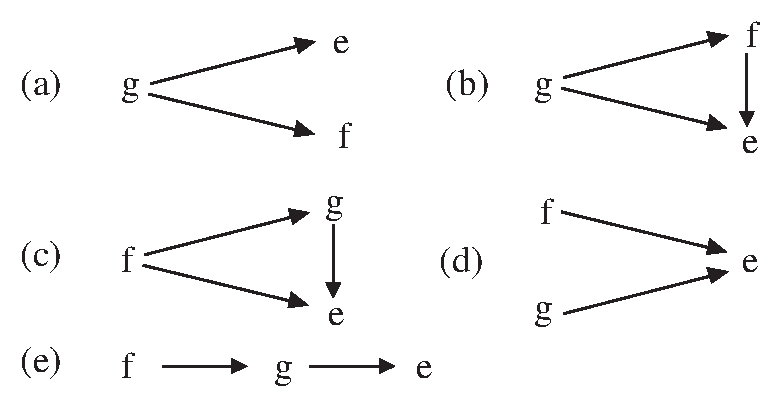
\includegraphics[scale=0.8]{figurer/fig9_1.pdf} 
 \caption{Ulike årsaksforhold}
	\label{fig:aarsaksforhold}
\end{figure}

For å klarlegge noen muligheter kan vi se på Figur~\ref{fig:aarsaksforhold}, som illustrerer
hvordan et tredje kjennetegn $g$ kan påvirke sammenhengen mellom to 
kjennetegn $e$ og $f$.  Pilene indikerer årsaksforhold som har en bestemt
 retning. Eksempelvis 
illustrerer Figur~\ref{fig:aarsaksforhold}a den mulighet at kjennetegn $g$ påvirker begge
kjennetegnene $e$ og $f$, mens disse ikke påvirker hverandre innbyrdes.
Dette betyr at en observert samvariasjon mellom $e$ og $f$ ikke gir
uttrykk for noen årsakssammenheng, den kan forklares ved den
``utenforliggende" faktor $g$.  I Figur~\ref{fig:aarsaksforhold}b har vi i tillegg den muligheten
at kjennetegn $g$ også påvirker $e$ via $f$, og hvor også
$f$ muligens har en egenvirkning på $e$.  Tolk selv Figur~\ref{fig:aarsaksforhold}c-e.  

Dersom man, ut fra observasjoner, har funnet samvariasjon (eller mangel
på samvariasjon) mellom $e$ og $f$, bør man være forsiktig
med å trekke generelle konklusjoner ut fra dette alene.  Ved 
innføring av et tredje kjennetegn $g$ kan situasjonen fortone seg noe
annerledes.  La oss se på en konkret problemstilling:\\

\begin{eksempel}{Kortkort}
\begin{table}[ht] \centering 
\begin{tabular}{l|rr|r|rr|r}
  &\multicolumn{3}{c|}{Konfeksjon} &\multicolumn{3}{c}{Elektro}\\ \cline{2-7}
           &      Kont. & Kort & Sum   &   Kont. & Kort & Sum  \\  \hline
Kvinne     &       70   &   40  & 110   &    15   &   15  &  30  \\
Mann       &       25   &   25  &  50   &    25   &   35  &  60  \\  \hline
Sum        &       95   &   65  & 160   &    40   &   50  &  90  \\  \hline
\end{tabular}
\caption{Kortbruk-data}
\label{tab:kortbruk} % Tabell_9
\end{table}

\begin{table}[ht] \centering
\begin{tabular}{l|rr|r}
          &   Konfeksjon  &  Elektro   &   Sum  \\  \hline
Kvinne    &       110     &     30     &   140  \\
Mann      &        50     &     60     &   110  \\  \hline
Sum       &       160     &     90     &   250  \\  \hline
\end{tabular}
\caption{Kortbruk-marginale data}
\label{tab:kortbruk_marginal_kjonn} % Tabell_10
\end{table}

\begin{table}[h] \centering 
\begin{tabular}{l|rr|r}
          &   Konfeksjon  &  Elektro   &   Sum  \\  \hline
Kontant   &       95      &     40     &   135  \\ 
Kort      &       65      &     50     &   115  \\  \hline
Sum       &      160      &     90     &   250  \\  \hline
\end{tabular}
\caption{Kortbruk-marginale data}
\label{tab:kortbruk_marginal} % Tabell_11
\end{table}
La situasjonen være som i Eksempel 2.  Av Tabell~\ref{tab:linjevise} ser vi at 
tilbøyeligheten til å bruke kort er betydelig mindre blant kvinner
enn blant menn.  Gir dette grunn til å påstå at kvinner er
mindre ``kortbevisste" enn menn?  Neppe!  Dette innser vi raskt dersom
vi bringer andre kjennetegn inn i diskusjonen.  Varehuset består av
to avdelinger, konfeksjon og elektrisk utstyr.  La oss tenke oss at
tallmaterialet er klassifisert mhp. de tre kjennetegnene betalingsform
($e$), kjønn ($f$) og avdeling ($g$).  Anta at de nødvendige 
data er gitt i Tabell~\ref{tab:kortbruk}.  \footnote{Ved å legge Elektrotabellen
over Konfeksjonstabellen får vi en tredimensjonal $2\times 2\times 2$ 
tabell.}
Ut fra denne tabell får vi to nye $2\times 2$ tabeller, nemlig
Tabell~\ref{tab:kortbruk_marginal_kjonn} og~\ref{tab:kortbruk_marginal} 
i tillegg til Tabell~\ref{tab:data}.

Disse resultatene rommer mange tolkningsmuligheter.  Mest 
påfallende er at kjennetegnene kjønn og avdeling viser betydelig 
grad av samvariasjon (Tabell~\ref{tab:kortbruk_marginal_kjonn}).  Vurderer vi så samvariasjonen
mellom kjennetegnene kjønn og betalingsmåte innen hver avdeling
(Tabell~\ref{tab:kortbruk}), ser vi at kjennetegnet avdeling  i noen grad kan forklare
den samvariasjon vi observerte i Tabell~\ref{tab:data}.  Følgende forklaring er
mulig:  I konfeksjonsavdelingen handler mesteparten av kundene for mindre
beløp hvor tilbøyeligheten til å bruke kort er liten, mens 
elektroavdelingen selger hovedsakelig større for\-bruks\-gjen\-stander
hvor kortbruk er mer vanlig.  I en situasjon hvor kvinnene viser større
tilbøyelighet til å være kunde i konfeksjonsavdelingen enn i
elektroavdelingen vil Tabell~\ref{tab:data} alene ikke være særlig
informativ.  De observerte data kan forklares ut fra årsaksskjemaet
gitt i Figur~\ref{fig:aarsaksforhold}c, der kjennetegnet kvinne ($f$) påvirker betalingsform
($e$) via avdeling ($g$), men trolig også direkte.  Det siste er 
altså en effekt som er til stede selv etter at vi har tatt hensyn
til forskjeller som skyldes avdeling.  Betyr en slik effekt at kvinner
likevel må sies å være mindre kortbevisste enn menn?  Ikke
ubetinget!  Ytterligere innsikt kan vi oppnå ved å utvide
diskusjonen til enda flere kjennetegn, mest interessant er kanskje
yrkesstatus.  Hvis flere menn enn kvinner er yrkesaktive,
og disse får lønn via lønnskonto i bank (og dermed kort
 opp i hendene), vil dette kunne forklare en stor del av forskjellen
mellom mann og kvinne. Årsakskjeden er kanskje som i Figur~\ref{fig:aarsaksforhold}e hvor 
kjennetegnet yrkesstatus er $g$.  Et utsagn om at kvinner, fordi de er
kvinner, viser mindre tilbøyelighet til kortbruk enn menn, vil
imidlertid lett kunne misforstås.  Dersom en sammenlignet kategoriene
yrkeskvinne og yrkesmann m.h.t. kortbruk, kan det tenkes at det ikke
er noen forskjell i det hele tatt, ja endog at sammenhengen går i
motsatt retning, dvs. yrkeskvinnene er mer ``kortbevisste" enn mennene.
For ytterligere spekulasjoner se Oppgave~4.
\end{eksempel}

Ved analyse av samvariasjon mellom to kjennetegn og innføring av et
tredje kan man oppleve følgende:

\begin{itemize}
\item En observert samvariasjon mellom to kjennetegn kan ``forklares bort"
      ved innføring av et tredje kjennetegn.
\item En observert samvariasjon mellom to kjennetegn er fremdeles til
      stede etter at et tredje kjennetegn forklarer en del av 
      samvariasjonen mellom de to første.
\item Det er samvariasjon mellom de to kjennetegn også etter at et 
      tredje kjennetegn innføres, men samvariasjon går nå i
      motsatt retning.
\item To kjennetegn som vurdert for seg synes uavhengige, viser sam\-varia\-sjon
      dersom man tolker observasjoner i relasjon til et tredje kjennetegn.
\end{itemize}

La oss gi eksempler på hver av disse, for korthets skyld utelater
vi konkrete tall.\\


\begin{eksempel}{Storker og fødsler}
I Danmark observerte man før i tiden at hyppigheten av storker var
større i områder med mange barn enn i områder med få barn.
Få vil likevel påstå at det var noe årsaksforhold mellom
kjennetegn barn ($e$) og stork ($f$).  En utenforliggende faktor kan
være folketetthet ($g$). En stor folke\-tett\-het medfører på
den ene siden mange barn, på den andre siden mange hus med piper
som gir plass for hekkende stork.  Dette tankemønster svarer til
Figur~\ref{fig:aarsaksforhold}a.  Folketetthet er muligens en forklarende årsak.
\end{eksempel}

\begin{eksempel}{Røking og lungekreft}
Det er observert positiv samvariasjon mellom lungekreft ($e$) og 
røking ($f$).  Dersom man innfører urbaniseringsgrad som et tredje
kjennetegn ($g$), viser det seg at hyppigheten av lungekreft er større
blant røkere enn ikke-røkere både i områder med lav og høy
urbanisering.  Videre viser det seg at urbane røkere viser høyere
tendens til lungekreft enn ikke-urbane røkere.  Det samme er tilfelle
for ikke-røkere.  Dette synes å indikere at både kjennetegnet
røking og urbanisering kan påvise lungekreft.  Det observerte
resultat kan muligens forklares ved Figur~\ref{fig:aarsaksforhold}d eller 
kanskje Figur~\ref{fig:aarsaksforhold}b.  En
av grunnene til at det gikk lenge før røking ble allment akseptert
som en vanlig årsak til lungekreft var diskusjonen om hvorvidt det
ikke fantes andre utløsende faktorer som kunne forklare den påviste
samvariasjon.
\end{eksempel}

\begin{eksempel}{Vær og avling}
I et tallmateriale hvor kjennetegnene avling ($e$), og temperatur ($f$)
og nedbør ($g$) er observert i suksessive år (kategorier lav, høy)
fant man en ne\-ga\-tiv samvariasjon mellom temperatur og avling.  Dette var
noe over\-raskende idet man forestilte seg at varm vekstperiode var godt
for årsveksten.  Nå viste det seg at nedbør og avling
hadde positiv samvariasjon, mens nedbør og temperatur hadde negativ
samvariasjon.  Disse observasjoner kan forklares ved årsakskjeden i
Figur~\ref{fig:aarsaksforhold}c, slik at høy temperatur har posi\-tiv direkte effekt på
avling, men høy temperatur hører som regel sammen med lite regn,
som i sin tur gir dårlig avling.  Den observerte negative samvariasjon
mellom temperatur og avling kan skyldes at denne indirekte effekten av
temperatur er større enn den direkte.  Ser man på årene med
gjennomgående høy og lav nedbør hver for seg, viste det seg
at tem\-pera\-tur og avling i begge tilfeller hadde positiv samvariasjon,
altså for en gitt nedbørmengde er høy temperatur av det gode.
Faktum synes å være at i naturen er de to faktorene nedbør
og temperatur konkurrerende, mens de ikke vil være det i et drivhus,
hvor vi for å oppnå høy avling både har høy
temperatur og høy fuktighet.
\end{eksempel}

\begin{eksempel}{Alder og musikkinteresse}
I et tallmateriale er kjennetegnene interesse for klassisk musikk ($e$)
og alder ($f$) observert for et visst antall personer (kategorier lav,
høy).  Det viste seg at samvariasjon var såpass liten at vi er 
tilbøyelig til å si at alder ikke har noe å si for
interessen.  Dette kan imidlertid tilsløre interessante forhold.  La
oss i tillegg studere kjennetegnet utdanning ($g$) (kategori lav, høy).
Da viste det seg at dersom en betraktet personene med ``lav" og ``høy"
utdanning hver for seg, så hadde interesse og alder negativ
samvariasjon for den første kategorien, positiv samvariasjon for
den andre.  Når de to kategoriene slås sammen har disse effektene
oppveiet hverandre og forledet om til å tro at alder ikke påvirker
interesse for klassisk musikk.  Det er derfor likevel mulig at det foreligger
en årsakskjede som den i Figur~\ref{fig:aarsaksforhold}d.
\end{eksempel}

Vi har med de foregående eksempler ønsket å vise at tilsynelatende 
enkle datamaterialer kan gi rom for flere tolkningsmuligheter, og at det
foreligger betydelig fare for feiltolkninger dersom man studerer
samvariasjon mellom to kjennetegn isolert.  Det samme gjelder for parvis
sammenligning av en rekke kjennetegn.  Ideelt sett burde vi studere alle
de kjennetegn vi mener har betydning for problemet i sammenheng.  Vi
skjønner imidlertid at med fire kjennetegn eller mer blir
tolkningsmulighetene svært mange og analysen av dataene blir, dersom
vi skal gå fram som i Eksempel 7, snart uoversiktlig. 

Et tjenlig verktøy for analyse av kategoridata er basert på såkalte
{\em  loglineære modeller}.
Slike gir mulighet for analyse på en systematisk oversiktlig
måte, slik at vi best mulig er i stand til å fange opp 
særtrekk i datamaterialet, samt å avgjøre om disse 
kan skyldes tilfeldigheter eller ikke.


\section{Samvariasjon av målevariable}

En problemstilling av betydelig praktisk og prinsipiell interesse er:
Det foreligger en populasjon, og man er interessert i sammenhengen mellom
to variable i denne populasjonen.  Det er ofte ikke hensiktsmessig å
observere sammenhørende verdier for alle elementene i populasjonen.
I steden trekkes et utvalg.  En kan da foreta korrelasjonsberegninger
for observasjonene i utvalget og spørsmålet er i hvilken grad disse
kan danne utgangspunkt for generelle konklusjoner om korrelasjonen 
mellom de to variable i hele populasjonen. La oss nevne konkrete eksempler:

En økonom ønsker å studere sammenhengen mellom
inntekt og sparing i en bestemt yrkesgruppe (f.eks. registrerte revisorer)
på grunnlag av et utvalg fra yrkesgruppen.  En psykolog ønsker 
å studere i hvilken grad to tester (f.eks. en skriftlig 
intelligenstest og en praktisk test) gjennomgående måler det
samme.  Hun anvender testen på et utvalg av elever.

I det første eksemplet har vi en avgrenset populasjon der inntekt og
sparing kan tallfestes for alle personene i populasjonen, men vi kjenner
tallene bare for personene i utvalget.  I det andre eksemplet er populasjonen 
ikke avgrenset på samme vis, men kan i en viss forstand oppfattes som 
alle de som disse testene kan tenkes anvendt på.  Selv om det aldri
vil kunne foreligge tall fra tester av alle disse, er det fruktbart å
tenke seg en ``sann" simultan testskår fordeling.  Denne fordeling blir
ofte tenkt på som en sannsynlighetsfordeling, den angir sjansen for
at en tilfeldig utvalgt person har en bestemt kombinasjon av testskårer
på de to testene.  Hvilke konklusjoner kan vi trekke om korrelasjonen
i denne teoretiske fordelingen på grunnlag av den observerte 
korrelasjonen mellom testskårene for personene i utvalget?  Vi er
inte\-res\-serte i dette spørsmålet fordi den teoretiske korrelasjonen
gir uttrykk for den samvariasjon vi kan vente oss ved mer almen anvendelse
av testene.

Vi tenker oss at ($X, Y$) er et stokastisk variabelpar med en 
simultan sannsynlighetsfordeling, der samvariasjonen uttrykkes ved
korrelasjons\-koeffisienten $\rho = \rho(X, Y)$ (se Kapittel 5.6).  På
grunnlag av $n$ uavhengige observasjoner fra denne fordelingen

\[  (X_1, Y_1),  (X_2, Y_2), \ldots, (X_n, Y_n)    \]
beregner vi den empiriske korrelasjonskoeffisienten $R = R_{XY}$ gitt
ved (se Eksempel 1.8).

\[ R_{XY}=\frac{S_{XY}}{S_X\cdot S_Y}=
             \frac{\frac{1}{n}\sum_{i=1}^n (X_i-\bar{X})\cdot (Y_i-\bar{Y})}
    {\sqrt{\frac{1}{n}\sum_{i=1}^n {(X_i-\bar{X})}^2}\cdot
     \sqrt{\frac{1}{n}\sum_{i=1}^n {(Y_i-\bar{Y})}^2}} \]

Vi vil kunne bruke $R$ som en estimator for $\rho$, og som testobservator
til å teste hypoteser om $\rho$.  Spesielt ønsker vi å teste
hypotesen om ukorrelerte variable, dvs.

\[ H_0 : \rho=0 \mbox{\ \ mot \ \ } H_A : \rho \neq 0   \]
Forat ikke tilfeldigheter skal spille oss et puss, bestemmer vi en 
kritisk verdi $k$ slik at vi påstår $H_A$ først når
$\mid R \mid \geq k$.  Ønsker vi at testen skal ha et bestemt
signifikansnivå, trenger vi å vite sannsynlighetsfordelingen til
$R$ når $H_0$ er riktig.  Det er utarbeidet tabeller for
bestemmelse av $k$ (avhengig av $n$) for gitte signifikansnivåer.
Disse forutsetter at den simultane sannsynlighetsfordeling til ($X, Y$)
er såkalt {\em binormal}. Dette betyr at både $X$ og $Y$ er normalfordelte
og at også alle betingede fordelinger for $Y$ gitt $X$ (og $X$ gitt $Y$)
er normalfordelte. I en slik fordeling medfører $\rho$ = 0 at
$X$ og $Y$ er uavhengige, noe som ikke gjelder generelt (se Kapittel 5.6).
Under denne forutsetningen kan vi isteden ta utgangspunkt i 

\[  T=\frac{R}{\sqrt{1-R^2}}\sqrt{n-2}    \]
som, dersom $H_0$ er riktig, er $t$-fordelt med $n-2$ frihetsgrader, en
fordeling vi allerede har tabeller for.\\


\begin{eksempel}{To tester}
Det observeres en score på to tester; en for verbal forståelse
($X$) og en for analytisk evne ($Y$).  Anta at disse er observert for
9 individer:

\begin{center}
\begin{tabular}{lrrrrrrrrr}
Individ ($i$) :&   1  &  2  &  3  &  4  &  5  &  6  &  7  &  8  &  9 \\
Score ($X_i$) :&  28  & 33  & 37  & 31  & 32  & 26  & 35  & 36  & 30 \\ 
Score ($Y_i$) :&  30  & 23  & 34  & 39  & 33  & 28  & 29  & 38  & 24
\end{tabular}
\end{center}
Her blir korrelasjonskoeffisienten $R$=0.345, dvs. moderat positiv 
(lineær) samvariasjon (tegn spredningsdiagram!)  Vi ønsker å
teste om disse data gir grunnlag for å påstå at
korrelasjonen er ulik null i den populasjon som individene er trukket
fra, evt. alle som testen er tenkt brukt på.  Vi får

\[  T=\frac{0.345}{\sqrt{1-0.345^2}}\sqrt{9-2}=0.97    \]
som langt fra er tilstrekkelig til å påstå at $\rho \neq 0$
i den tenkte bivariate populasjonsfordelingen. $t$-tabellen med 7
frihetsgrader krever kritisk verdi lik 2.365 for en tosidig test med
5\% signifikansnivå.  En $R$ = 0.345 vil være signifikant ulik
null først når antall observasjoner er 33 eller flere.
\end{eksempel}

\noindent {\bf Merknad. } Dersom $(X,Y)$ er binormalt fordelt gjelder at

\[ ER\approx \rho \mbox{\ \ \ \ \ } \sigma (R)\approx \frac{1}{\sqrt{n-2}} \]
et resultat som kan brukes til å lage tilnærmede konfidensintervaller
for $\rho$.\\

Avslutningsvis gir vi et par reservasjoner mot ukritisk bruk av 
korrelasjonskoeffisienter:  I utgangspunktet måler $R$ bare graden
av lineær samvariasjon for observasjonene.  Generalisering til den
underliggende fordeling (populasjon) krever antakelser (binormalitet)
som er vanskelig å begripe, enn si sjekke, og som derfor ofte overses.
I mange situasjoner vil en være tjent med å bruke en såkalt
{\em rangkorrelasjonskoeffisient,} der observasjonene er erstattet med
ranger.  En slik fanger opp monoton ikke-lineær sam\-varia\-sjon, og 
hypotesetesting kan skje med mindre restriktive forutsetninger enn 
binormalitet.  For videreføring av dette tema må vi vise til annen
litteratur.

I situasjoner der en har en rekke variable hvor en på forhånd 
har liten kunnskap om mulige sammenhenger, er det lett å ty til 
korrelasjonsberegninger på observasjonene for å skaffe seg innsikt,
eventuelt avsløre årsaks\-sammenhenger.  Dette er en praksis som 
ikke bør følges uten en viss innsikt i de mulige feiltolkninger
som er tilstede:  Korrelasjonsberegninger kan aldri bevise 
årsakssammenhenger mellom to eller flere variable.  Observerte 
kor\-rela\-sjoner mellom to variable kan endre karakter når de studeres
i lys av andre variable (partiell korrelasjon).  Her gjelder de samme
reservasjoner som ved slutten av forrige avsnitt.


\section{Oppgaver}
\small
\begin{enumerate}
\item
Vis at i modellen for et $2\times 2$ eksperiment betyr uavhengighet at
\begin{eqnarray*}
   p_{11}/(p_{11}+p_{12})&=&p_{21}/(p_{21}+p_{22}) \\
   p_{11}/(p_{11}+p_{21})&=&p_{12}/(p_{12}+p_{22})   
\end{eqnarray*}
Gi konkret fortolkning av hver likhet og vis at begge er ekvivalent med 

\[ p_{11}p_{22}/p_{12}p_{21}=1  \]
Forklar at dersom vi erstatter likhetene med ulikheten større enn
(mindre enn), så svarer dette til positiv (negativ) samvariasjon.

\item
Test hypotesen om uavhengighet mellom kjønn og stemmetilbøyelighet
i Eksempel 3 ved å bruke den beskrevne kjikvadratmetoden.

\item 
\begin{itemize}
\item[(a)] Test hypotesen om uavhengighet i de tre marginale $2\times 2$
tabellene i Eksempel 7.  (Tabellene~\ref{tab:data}, 
\ref{tab:kortbruk_marginal_kjonn} og~\ref{tab:kortbruk_marginal}).
\item[(b)] Test hypotesen om uavhengighet mellom kjønn og 
betalingsmåte innen hver avdeling (Tabell~\ref{tab:kortbruk}).
\end{itemize}

\item
Diskuter hvorvidt kunnskaper om følgende forhold kan ha interesse for
å vurdere tallene i Eksempel 7 om kortbruk:
\begin{itemize}
\item[(a)] varenes kostende.
\item[(b)] mann og hustru handler gjennomgående sammen i 
Elektroavdelingen.
\item[(c)] menn handler gjennomgående stort i Konfeksjonsavdelingen.
\end{itemize}

\item
En bedrift har i lengre tid produsert en bestemt artikkel, men har den senere
tid erfart et økende antall reklamasjoner.  I et første forsøk
på å skaffe seg innsikt i forholdet har man tatt for seg de
$n$ = 100 siste reklamasjonene.  Disse blir klassifisert etter to 
kjennetegn reklamasjonstype $A, B$ eller $C$ og produksjonskjede 1, 2
eller 3.  Resultatet ble

\begin{center}
\begin{tabular}{l|ccc|c}
         &  Type A  &  Type B  &  Type C  &   Sum  \\  \hline
Kjede 1  &    29    &    8     &    9     &    46  \\
Kjede 2  &     9    &    4     &    6     &    19  \\
Kjede 3  &    10    &    8     &   17     &    35  \\  \hline
Sum      &    48    &   20     &   32     &   100  \\  \hline
\end{tabular}
\end{center}

\begin{itemize}
\item[(a)] Test hypotesen om at reklamasjonstype og produksjonskjede er
uav\-hengige kjennetegn.  Bruk 5\% signifikansnivå.
\item[(b)] Dersom hypotesen forkastes, forsøk å tolke tallene
så langt det synes rimelig.
\end{itemize}

\item
To bedrifter produserer samme artikkel som de leverer under hvert sitt
varemerke.  Begge bedrifter leverer tre kvalitetssorteringer $A, B$ og $C$,
men produksjonen foregår etter to ulike metoder.  Bedriftene
vurderer nå å markedsføre varen under samme varemerke, men
før dette gjøres vil en gjerne ha rede på om de to bedriftene
leverer varer med ulik kvalitetsfordeling (hvorfor?).  For å 
klargjøre dette har man valgt ut 50 tilfeldige artikler fra hver bedrift
som blir kvalitetssortert.  Resultatet ble:

\begin{center}
\begin{tabular}{l|cc|c}
            &  Fabrikk 1  &  Fabrikk 2   &   Sum  \\  \hline
Kvalitet A  &     20      &     12       &    32  \\  
Kvalitet B  &     19      &     31       &    50  \\
Kvalitet C  &     11      &      7       &    18  \\  \hline
Sum         &     50      &     50       &   100  \\  \hline
\end{tabular}
\end{center}

Gir dette materialet grunnlag for å påstå at de to bedrifter
produserer ulik kvalitetsfordeling?  Velg 5\% signifikansnivå.

\item
Ved en eksamen på en høyskole leverte $n$=210 studenter inn
sin besvarelse ved en eksamen i statistikk.  Etter sensuren sammenholdes
opplysninger om bestått/ikke bestått med linje fra videregående
 skole .  Resultatet ble (tallene er konstruerte)

\begin{center}
\begin{tabular}{l|ccc|c}
                 &  Linje 1  &  Linje 2  &  Linje 3   &   Sum  \\ \hline
Bestått      &    74     &    58     &    38      &   170  \\
Ikke bestått &    16     &    12     &    12      &    40  \\ \hline
Sum              &    90     &    70     &    50      &   210  \\ \hline
\end{tabular}
\end{center}

Test hypotesen om at prestasjonen er uavhengig av linje.  Beregn
$P$-verdien til det observerte resultat og avgi konklusjon dersom vi
krever 1\% signifikansnivå.

\item
En studentforening arrangerer ekskursjon til et ølbryggeri for de
nye studentene.  Av $n$=250 studentene deltok i alt 100, og disse
fordelte seg etter bosted slik:

\begin{center}
\begin{tabular}{l|cccc|c}
            &Østpå&Sørpå&Vestpå&Nordpå& Sum \\ \hline
Deltok      &    38      &   16       &  25      &  21      & 100 \\
Deltok ikke &    57      &   29       &  40      &  24      & 150 \\ \hline
Sum         &    95      &   45       &  65      &  45      & 250 \\ \hline
\end{tabular}
\end{center}
Tyder dette på at interessen er uavhengig av bosted?  Utfør en
test med signifikansnivå 5\%.

\item
En butikk har reklamert i lokalavisene for en tilbudsvare som også
tilbys ved reklamearrangement inne i butikken.  I alt $n$=600 kunder
er blitt intervjuet når de forlater butikken og spurt om de har
kjøpt tilbudsvaren eller ikke (kjennetegn $e$), om de har lest
avisreklamen for tilbudsvaren eller ikke ($g$), om de regner seg for
fast kunde eller ikke ($f$).  Anta at resultatet ble

\begin{center}
\begin{tabular}{l|rr|rr}
    &\multicolumn{2}{c|}{Fast kunde}&\multicolumn{2}{c}{Tilfeldig kunde}  \\
             & Kjøpt & Ikke kjøpt & Kjøpt & Ikke kjøpt  \\ \hline
Lest reklame &    85    &       39      &    98    &       57       \\
Ikke lest    &    10    &       16      &    52    &      243       \\ \hline
\end{tabular}
\end{center}

Analyser tallmaterialet med sikte på å belyse ulike sammenhenger
mellom kjennetegnene.  Hvilke(n) av årsakskjedene i Figur~\ref{fig:aarsaksforhold} er
forenlig med dette tallmaterialet?

\item
$\star$ Betrakt to indikatorvariable $I$ og $J$ med simultan 
sannsynlighetsfordeling

\[ P[(I=i)\cap (J=j)]=p_{ij}  \]
for $i$=0,1 og $j$=0,1.  Vis at korrelasjonskoeffisienten mellom $I$ 
og $J$ er gitt ved (se Oppgave~\ref*{kap:stokastiske}.29)

\[ \rho =\frac{p_{00}p_{11}-p_{01}p_{10}}
    {\sqrt{(p_{00}+p_{01})(p_{10}+p_{11})(p_{00}+p_{10})(p_{01}+p_{11})}} \]
Bruk dette til å motivere det mål for samvariasjon i en
$2\times 2$ tabell som er gitt i teksten.

\item
I modellen for $2\times 2$ eksperimenter betrakt kryssproduktforholdet
$K = p_{11}p_{22}/ p_{12}p_{21}$.  Forklar at den såkalte 
Gammakoeffisienten

\[ \gamma =\frac{K-1}{K+1}=
            \frac{p_{11}p_{22}-p_{12}p_{21}}{p_{11}p_{22}+p_{12}p_{21}} \]
kan tjene som et mål for samvariasjon. Hva betyr det at \\
(a) $\gamma$ =0 \ \ \      (b) $\gamma$ =$-$1 \ \ \   (c) $\gamma$ = +1 .

\item
Beregn gammakoeffisienten $G$ for samvariasjon i følgende 
kontingenstabeller:
\begin{center}
\begin{tabular}{|rrr|rrr|rrr|} \hline
(a)&20&20&(b)&30&20&(c)&20&30\\ 
   &30&30&   &20&30&   &30&20\\ \hline
(d)&20&10&(e)&10& 5&(f)&10&40\\
   &30&40&   &40&45&   &40&50\\ \hline
\end{tabular}
\end{center}
Kommenter resultatene.

\item
\begin{itemize}
\item[(a)] Vis at for $2\times 2$ tabeller gjelder sammenhengen 
$Q = nR^2$ mellom kjikvadratobservatoren $Q$ og korrelasjonsmålet
$R$ gitt i teksten.
\item[(b)] Beregn $R$ for situasjonene ($a$) - ($f$) i Oppgave~12.
\end{itemize}

\item
Test om beregnet korrelasjonskoeffisient mellom karakteren i
bedrifts\-økonomi og samfunnsøkonomi i Eksempel 1.8 er signifikant
forskjellig fra null.  Forklar at det er rimelig å benytte en
ensidig test her.  Hva er populasjonen det generaliseres til?  Kunne
en isteden ha brukt kjikvadrattest?

\item
Vis at minste kvadraters regresjonslinjen for $Y$ mhp. $X$ faller sammen
med minste kvadraters regresjonslinjen for $X$ mhp. $Y$ hvis og bare 
hvis $R_{XY} = \pm 1$.

\item
Ved en skole avholdes eksamen i to obligatoriske fag hvor kunnskaper i
hvert av fagene antas å ha en viss overføringsverdi til det andre.  
Anta at 10 studenter deltok ved begge eksamener, og deres karakterer
målt på en 0 til 9 skala ble 

\begin{center}
\begin{tabular}{ccccccccccc}
 $X$:  &  4 & 2 & 8 & 5 & 6 & 7 & 0 & 5 & 6 & 7  \\
 $Y$:  &  4 & 0 & 5 & 4 & 2 & 6 & 1 & 5 & 7 & 6  \\
\end{tabular}
\end{center}

\begin{itemize}
\item[(a)] Tegn spredningsdiagram.
\item[(b)] Beregn $\bar{X}, \bar{Y}, S_X, S_Y, S_{XY}$ og $R_{XY}$.
\item[(c)] Bestem minste kvadraters regresjonslinje for $Y$ mhp. $X$
           og $X$ mhp. $Y$, og tegn begge inn i spredningsdiagrammet.
\item[(d)] To studenter hadde karakterene $X$=2 og $X$=7 ved den første
           eksamen, men møtte ikke til den andre pga. sykdom.  Gi en 
           prediksjon for deres respektive prestasjoner dersom de hadde 
           møtt.
\item[(e)] To studenter møtte ikke til den første eksamen pga.
           sykdom, men fikk karakter $Y$=2 og $Y$=7 ved den andre.  Gi en
           prediksjon for deres prestasjoner dersom de hadde møtt.
\item[(f)] Drøft om det er rimelig å bruke to ulike linjer i
           ($d$) og ($e$) til prognoseformål, eller om det ville være
           bedre å bruke en felles linje fastlagt ut fra 
           spredningsdiagrammet.
\end{itemize}
\item
Gitt $n$ observasjonspar ($X_i, Y_i$) $i = 1,2,\ldots, n$.  Anta at det 
er foretatt en lineær skalaendring av observasjonene, dvs. at vi
isteden observerer ($V_i, W_i$) $i = 1,2,\ldots, n$, der $V_i = a+bX_i$
og $W_i = c+dY_i$ (Jfr. Oppgave~\ref*{kap:stokastiske}.29).

\begin{itemize}
\item[(a)] Vis at $S^2_V = b^2\cdot S^2_X$ og $S^2_W = d^2\cdot S^2_Y$
\item[(b)] Vis at $S_{VW} = bd\cdot S_{XY}$
\item[(c)] Vis at $R_{VW} = \pm R_{XY}$ med positivt tegn dersom $b$
og $d$ har samme fortegn.
\end{itemize}

\end{enumerate}
\normalsize

